\subsection{Résultats du projet APEX BES}

\subsubsection{Résultats principaux}

Les acquisitions APEX sont correctement reçues et exploitables côté station sol. Les essais mettent en évidence :
\begin{itemize}
    \item une cohérence qualitative entre la cinématique observée (trajectoire vidéo) et les tendances des signaux \acrshort{IMU},
    \item une limitation dans le cas où la cinématique imposée reste trop lente : les variations d’accélération et de vitesse
    angulaire deviennent proches du niveau de bruit, ce qui réduit la discriminabilité,
    \item à l’inverse, lors d’une excitation plus marquée (mouvement plus brusque ou sollicitation volontaire),
    l’apparition de pics sur les courbes station sol confirme le bon fonctionnement de la chaîne d’acquisition et de transmission.
\end{itemize}

\begin{figure}[H]
    \centering
    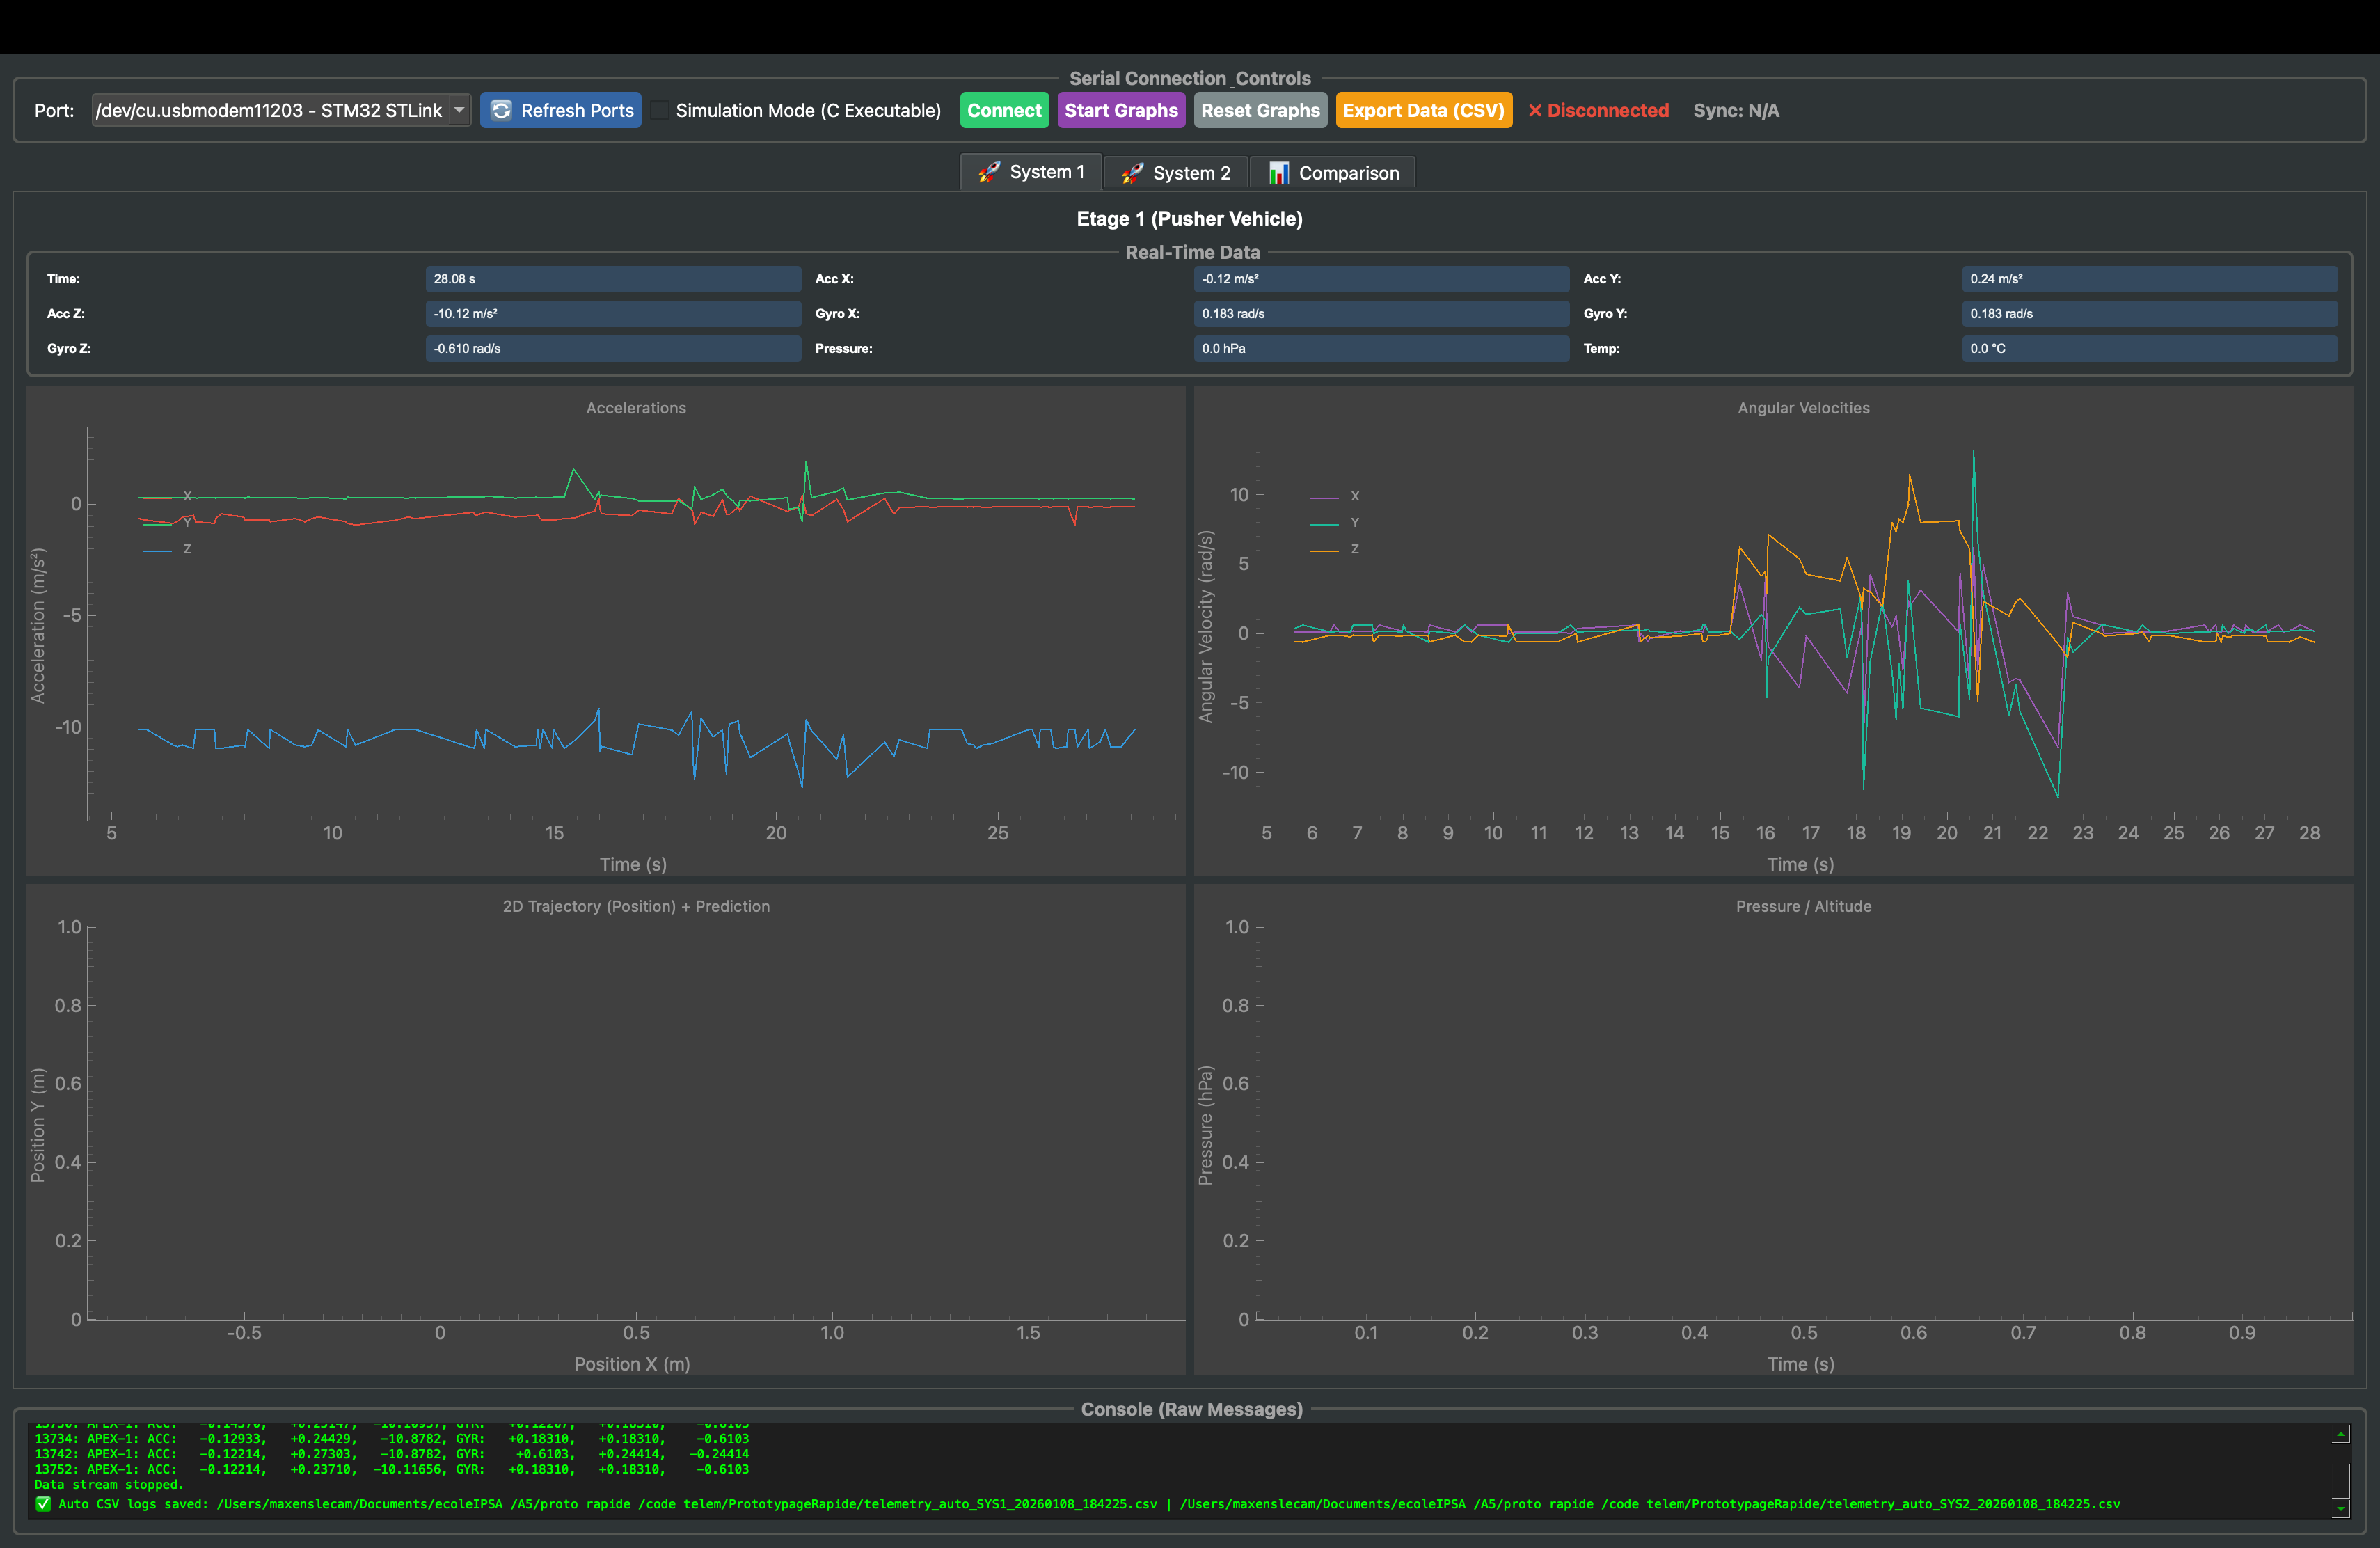
\includegraphics[width=0.8\textwidth]{figures/apex_bes/Capture d’écran 2026-01-08 à 18.46.17.png}
    \caption{Affichage des données d'APEX reçu par télémesure et affiché en directe}
    \label{fig:apex_bes_fig04}
\end{figure}

\subsubsection{Discussion}

Le banc démontre l’intérêt d’un support d’essai instrumenté : les véhicules permettent de rejouer des scénarios de mouvement, de
calibrer l’exploitation des mesures et d’identifier les limites liées au niveau d’excitation. Deux points ressortent :
\begin{itemize}
    \item \textbf{Validation fonctionnelle :} la chaîne APEX (acquisition, transmission, affichage) est opérationnelle.
    \item \textbf{Niveau d’excitation requis :} pour quantifier finement l’accord vidéo avec \acrshort{IMU}, il est nécessaire
    de forcer une dynamique suffisante (accélérations/rotations) au-delà du bruit et des biais.
\end{itemize}

\subsubsection{Conclusion de l’essai}

Le banc développé (deux véhicules instrumentés) a permis de mettre en place une procédure de test complète, reproductible et
directement exploitable pour qualifier la chaîne APEX. Néanmoins, la cinématique réellement obtenue durant les essais reste
trop lente pour mettre en évidence de manière concluante une corrélation fine entre la trajectoire reconstruite par vidéo et les
grandeurs inertielle (accélérations et vitesses angulaires) : les variations attendues se confondent majoritairement avec le
niveau de bruit et les biais de mesure.\\

En revanche, l’essai valide un point essentiel : la \textbf{transmission est fonctionnelle}. Les données issues de
l’\acrshort{IMU} sont bien acquises et envoyées à la station sol, puis affichées et tracées en temps réel. Cela est confirmé par
l’observation de \textbf{pics et variations nettes} sur les courbes lorsque les véhicules sont excités volontairement, notamment
lors des sollicitations de type « secouement » simulant une réaction d’évitement. Ces signatures dynamiques, visibles
immédiatement côté station sol, démontrent que la chaîne acquisition $\rightarrow$ transmission $\rightarrow$ réception
$\rightarrow$ visualisation fonctionne correctement et avec une réactivité compatible avec un suivi en temps réel.\\

Les conclusions présentées ici se limitent volontairement au périmètre de validation obtenu : fonctionnalité de la
chaîne de transmission et détectabilité d’excitations dynamiques, sans prétendre à une validation quantitative complète dans le
cas de déplacements lents.

\newpage
